
\documentclass[12pt]{article}
\usepackage[a4paper, total={6.5in, 9in}]{geometry}
\usepackage{import}

\import{./}{macros}


\title{
    % UW Mech/Tron Eng Logo
    
\includegraphics[width=0.75\linewidth]{resources/uwaterloo_mechanical_and_mechatronics_engineering/UWaterloo_Mechanical_Mechatronics_Eng_Logo_vert_rgb.png}
    \\~\\
    \bf{
        ME 546 - Lab 3 \\
        Complete Sensor Fusion System
    }
    \sepline
    \\~\\
    % \large Subtitle Something Something
}
\author{
    \begin{center}
        \begin{tabular}{ c c }
        William Ancich & Austin Milne \\
        \multicolumn{2}{ c }{Jude Bennett} \\
        \end{tabular}
    \end{center}
}
\date{March 03, 2024}


\begin{document}
\pagenumbering{gobble}
\maketitle
\vfill % Use this instead of clearpage to keep Abstract on the front page
% \clearpage % Use this instead of vfill to put abstract on 2nd page
% \pagenumbering{roman} % Uncomment pagenumbering under abstract if abstract is on 2nd page.
\begin{abstract}
    \centering\noindent
    This report was prepared for Prof. Arash Araami as part of the ME 546 - Multi Sensor Data Fusion Course. The goal of this lab is to fuse the readings of multiple different types of sensors using Bayesian fusing.
\end{abstract}

\clearpage
\pagenumbering{roman} % Comment pagenumbering above abstract if abstract is on 1st page.

\tableofcontents
\clearpage
% \vspace{1cm}
% \sepline
% \vspace{1cm}

\listoftables % Comment out if no tables.
\listoffigures % Comment out if no figures.
%% NEEDS LIST OF EQUATIONS!!
\lstlistoflistings % Comment out if there are no listings.

% Experiment Setup ──────────────────────────────────────────────────────────────── %
\clearpage
\pagenumbering{arabic} % Reset page number to arabic numbers, restart numbering.
\section{Experiment Setup} \label{sec:setup}

The experiment was prepared as outlined in the Lab Manual \cite{lab-manual}. Due to there being issues with some of the sensors on the lab, an alternate set of sensors were used than those prescribed:

\begin{itemize}
    \item 2 Long Distance IR Sensors (Sharp GP2Y0A02YK0F)
    \item 2 Short Distance IR Sensors (Sharp GP2Y0A41SK0F)
\end{itemize}

\noindent The Long and Short sensors were kept together. This was done to avoid the potential issue the sensors physically interfering with the others' views. Due to the vastly different reading range, the short sensor would need to be much closer than the long sensor and could physically block its view, returning uncharacteristic measurements. The final configuration had the two short sensors reading in the $Y$ direction and the two long sensors reading in the $X$ direction.

\begin{figure}[H]
    \centering
    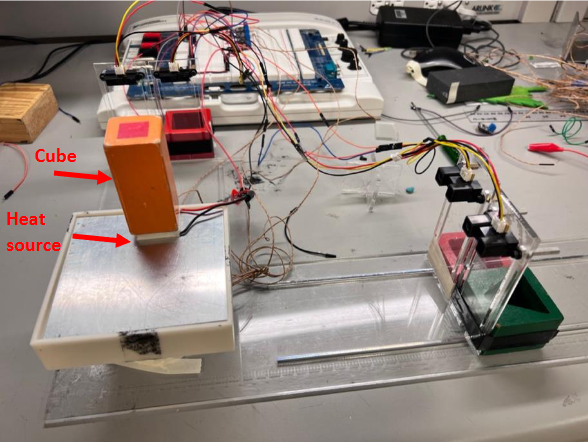
\includegraphics[width=0.75\linewidth]{images/setup.png}
    \caption{Example Setup \cite{lab-manual}}
    \label{fig:setup}
\end{figure}

Before collecting the training data, a series of measurements were taken with the IR sensors to later calibrate them. Each sensor was measured at 6 or 7 distances, 2 closer than the plates edges, 1 at the closest edge, 1 at the center, 1 at the furthest edge, and 1 or 2 past the furthest edge. This allowed for a general profiling of the IR sensors along with specific data for the range to be measured in.

For the training data, 9 points were selected along the grid. Four points at the corners, 1 at the center, and the remaining 4 in the intermediaries between the previous points. The location of the block was measured for each positional reading. They are displayed in figure \ref{fig:experimental-layout}. The points are numbered as shown in figure \ref{fig:layout}, such that 1, 3, 7, and 9 are the corner measurements.

\begin{figure}[H]
    \centering
    \begin{tabular}{c|c|c}
        1 & 2 & 3 \\ \hline
        4 & 5 & 6 \\ \hline
        7 & 8 & 9 \\
    \end{tabular}
    \caption{Training Measurement Layout}
    \label{fig:layout}
\end{figure}

\begin{figure}[H]
    \centering
    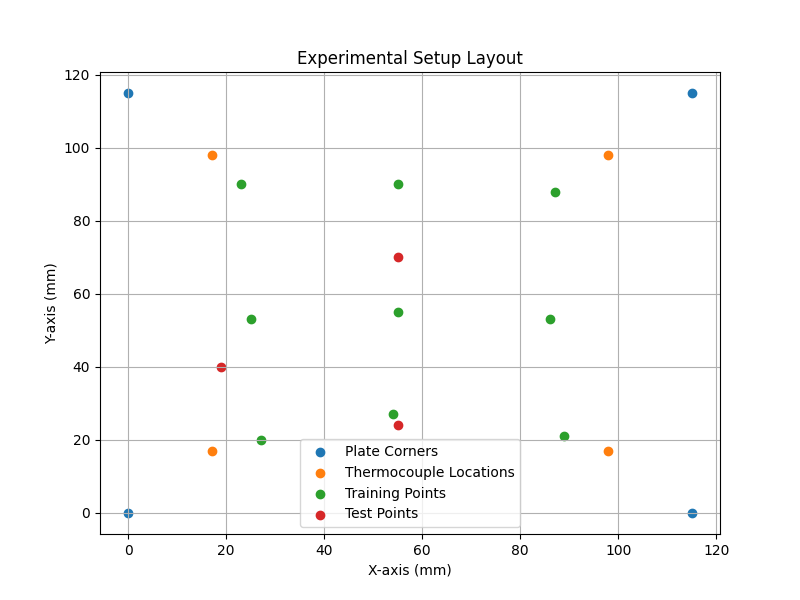
\includegraphics[width=\linewidth]{images/Experimental Setup Layout.png}
    \caption{Experimental Setup Layout}
    \label{fig:experimental-layout} % Label is defined below the content, to place it below the image.
\end{figure}

After training data was collected, 3 additional points were collected for later testing of the developed model. 1 measurement was taken in a previously trained position, the other 2 were taken in intermediary positions that do not exist in the training set. This was done to compare the performance of the model on known and unknown states. The exact locations of the test points are listed in table \ref{tab:test_points}.

\begin{table}[H]
    \centering
    \caption{Test Point Locations}
    \label{tab:test_points}
    \begin{tabular}{|c|cc|}
        \hline
        Point & X (mm) & Y (mm) \\ \hline
        #1 & 55 & 24 \\
        #2 & 19 & 40 \\
        #3 & 55 & 70 \\ \hline
    \end{tabular}
\end{table}

Between all measurements requiring the thermocouples, the aluminum plate was removed from the fixture. The plate was shaken in the air for 30-45 seconds to accelerate the heat dissipation and return it to room temperature. Each of the thermocouples was raised above the necessary height, and then the plate was placed on top of them and tapped down to ensure full contact with all 4 sensors. The Peltier cell was then very gently placed on the aluminum plate as to not move the thermocouples and the wooden block was place atop the cell.

% Sensor Calibration ──────────────────────────────────────────────────────────────── %
\section{Sensor Calibration} \label{sec:calib}

\subsection{IR Sensor Profiling} \label{sec:ir-calib}

As mentioned in Section \ref{sec:setup}, measurements were taken on both the short and long range sensors at a variety of distances. Figure \ref{fig:raw-short-ir} and \ref{fig:raw-long-ir} show the raw voltage measurements for the short and long range sensors, respectively. The voltage graphs show a consistent and uniform voltage reading for each of the sensors, showing that the sensors were wired correctly and behaved as expected.

\begin{figure}[H]
    \centering
    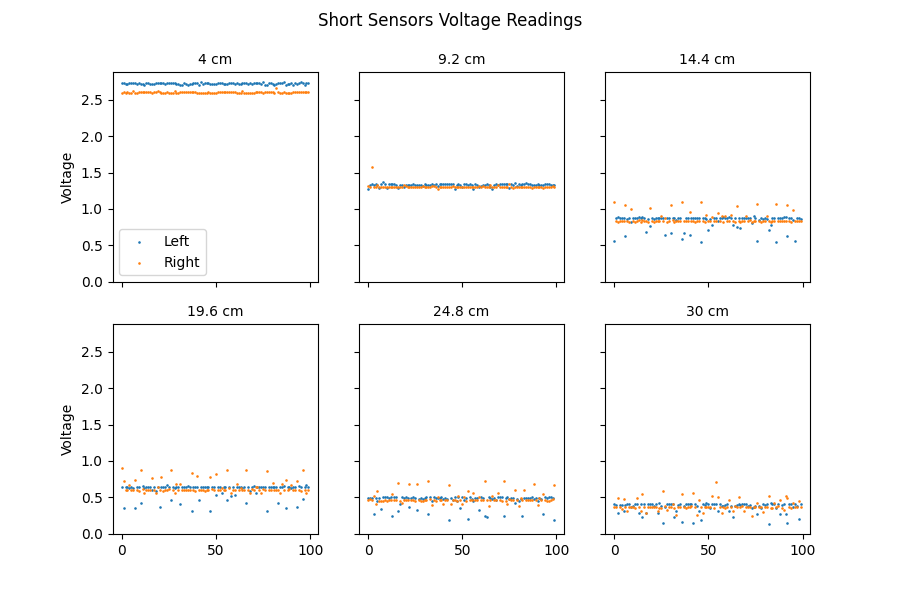
\includegraphics[width=\linewidth]{images/Short Sensors Voltage Readings.png}
    \caption{Short IR Sensors Raw Voltage Readings}
    \label{fig:raw-short-ir} % Label is defined below the content, to place it below the image.
\end{figure}

\begin{figure}[H]
    \centering
    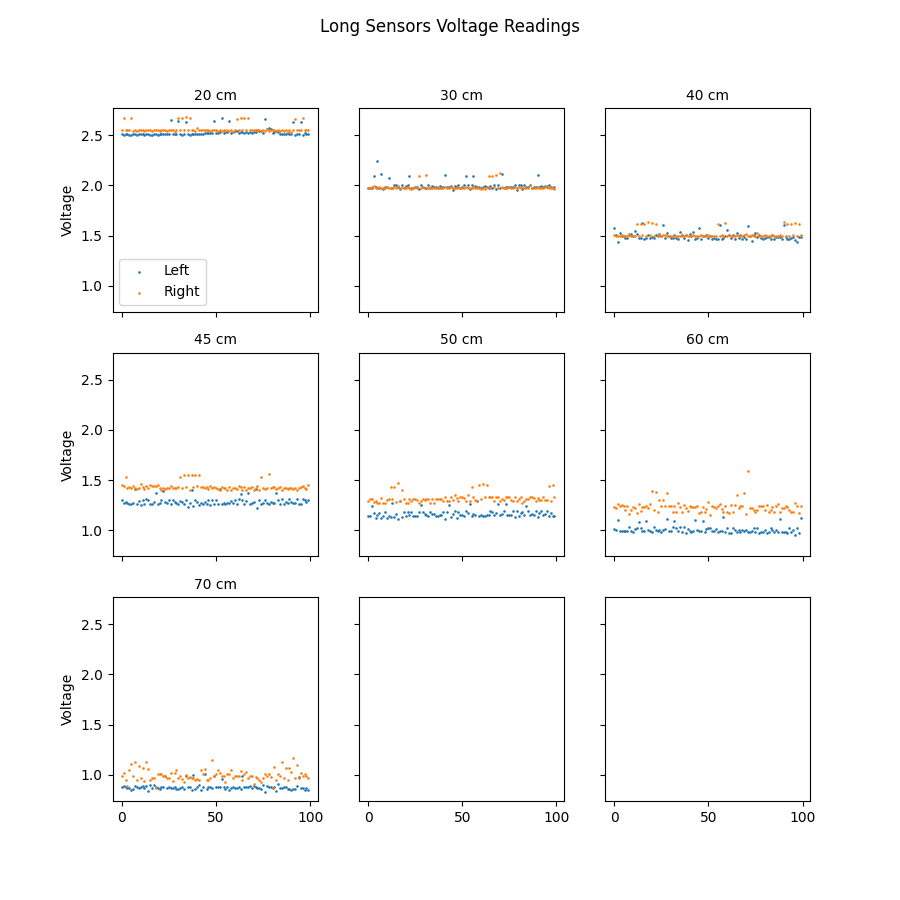
\includegraphics[width=\linewidth]{images/Long Sensors Voltage Readings.png}
    \caption{Long IR Sensors Raw Voltage Readings}
    \label{fig:raw-long-ir} % Label is defined below the content, to place it below the image.
\end{figure}

Data for each of the sensors was used to create a Voltage and Distance relation. Regression was done using as inverse relationship as previously proven in Lab 1 \cite{lab-1}, as show in equation \ref{eqn:inverse}. The regressions and resultant parameters are shown for each IR sensor in figure \ref{fig:regression-ir}.

\begin{gather}
    \label{eqn:inverse}
    D = a \times V + b
\end{gather}


\begin{figure}[H]
    \centering
    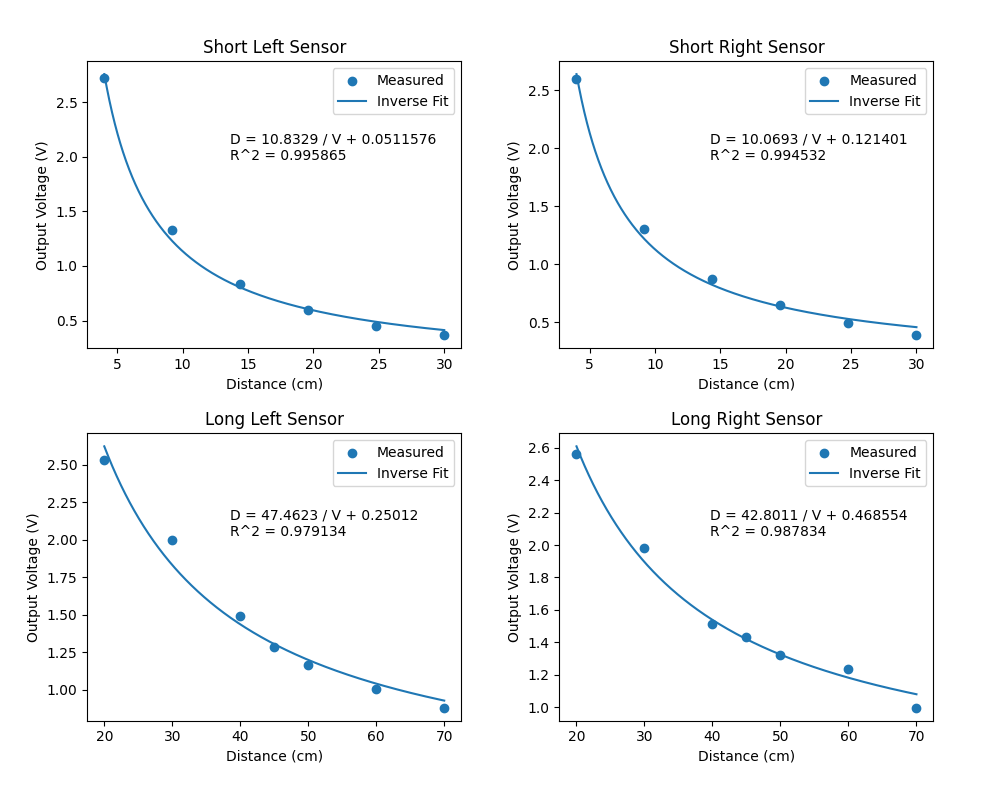
\includegraphics[width=\linewidth]{images/IR Sensor Fits.png}
    \caption{IR Sensors Regression to Inverse Relationship}
    \label{fig:regression-ir} % Label is defined below the content, to place it below the image.
\end{figure}


\subsection{Thermocouple Profiling} \label{sec:tc-calib}

As mentioned in Section \ref{sec:setup}, measurements were taken with all thermocouples with the heat source placed at a variety of positions. Figure \ref{fig:raw-thermocouple} shows the raw voltage measurements for each thermocouple, at each position in the training set. The voltage graphs show a consistent and uniform voltage reading for each of the thermocouples, as was expected behavior for the sensor at steady state operation.

\begin{figure}[H]
    \centering
    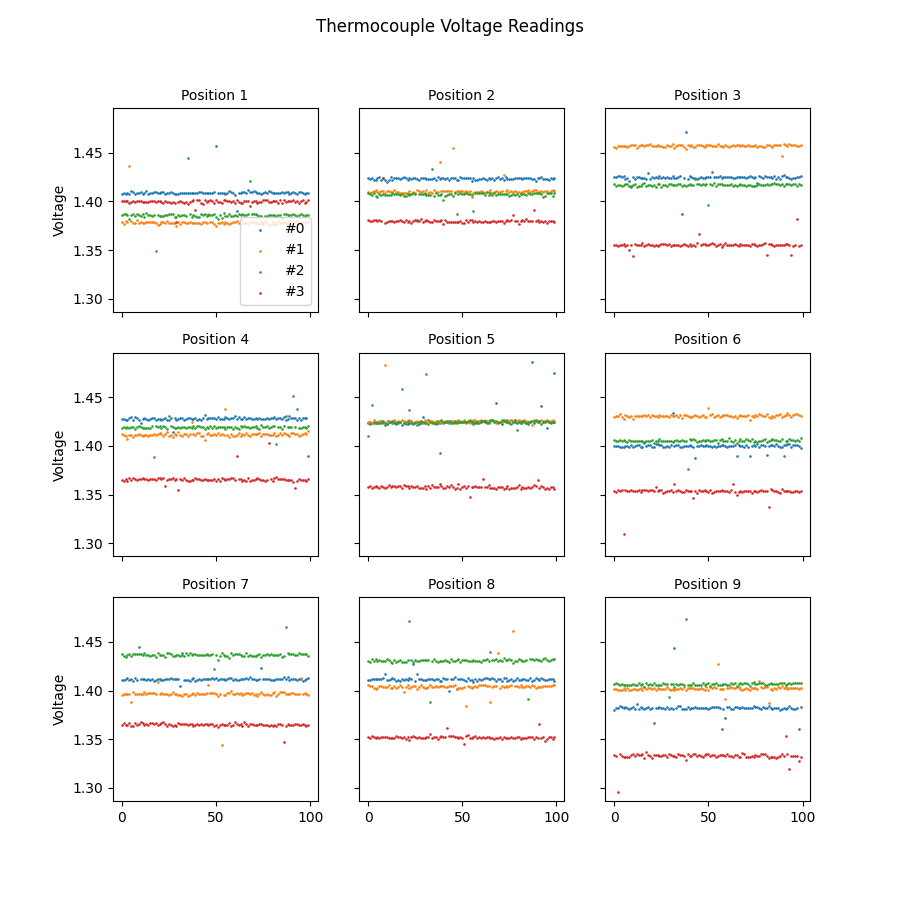
\includegraphics[width=\linewidth]{images/Thermocouple Voltage Readings.png}
    \caption{Thermocouple Raw Voltage Readings}
    \label{fig:raw-thermocouple} % Label is defined below the content, to place it below the image.
\end{figure}

As the thermocouple was a sensor that had not been used prior to this lab, modelling the thermocouple was first required. The desired model needed to establish the relationship between thermocouple temperature readings and the distance between a thermocouple and the heat source. As with the IR sensors, the voltages readings obtained earlier were averaged mitigate the effect of sensor noise. Then, the mean output voltages from the thermocouples were substituted into equation \ref{eqn:tc_conv} from the lab manual \cite{lab-manual} to obtain corresponding temperature readings.

\begin{gather}
    \label{eqn:tc_conv}
    T = \frac{V_{\text{out}} - 1.25}{0.005}
\end{gather}

To establish a relationship between distance and temperature, least squares were used to fit functions (linear, inverse, quadratic, cubic) to the test data. These functions were then plotted (as shown in figure \ref{fig:compare-tc}) and the coefficient of determination was evaluated for each of these functions (using the true and predicted distance values) to assess which model was the most accurate. At this point it was noted that the relationship between temperature and distance was reversed for thermocouple #4, indicating that it was wired in reverse during data collection.

\begin{figure}[H]
    \centering
    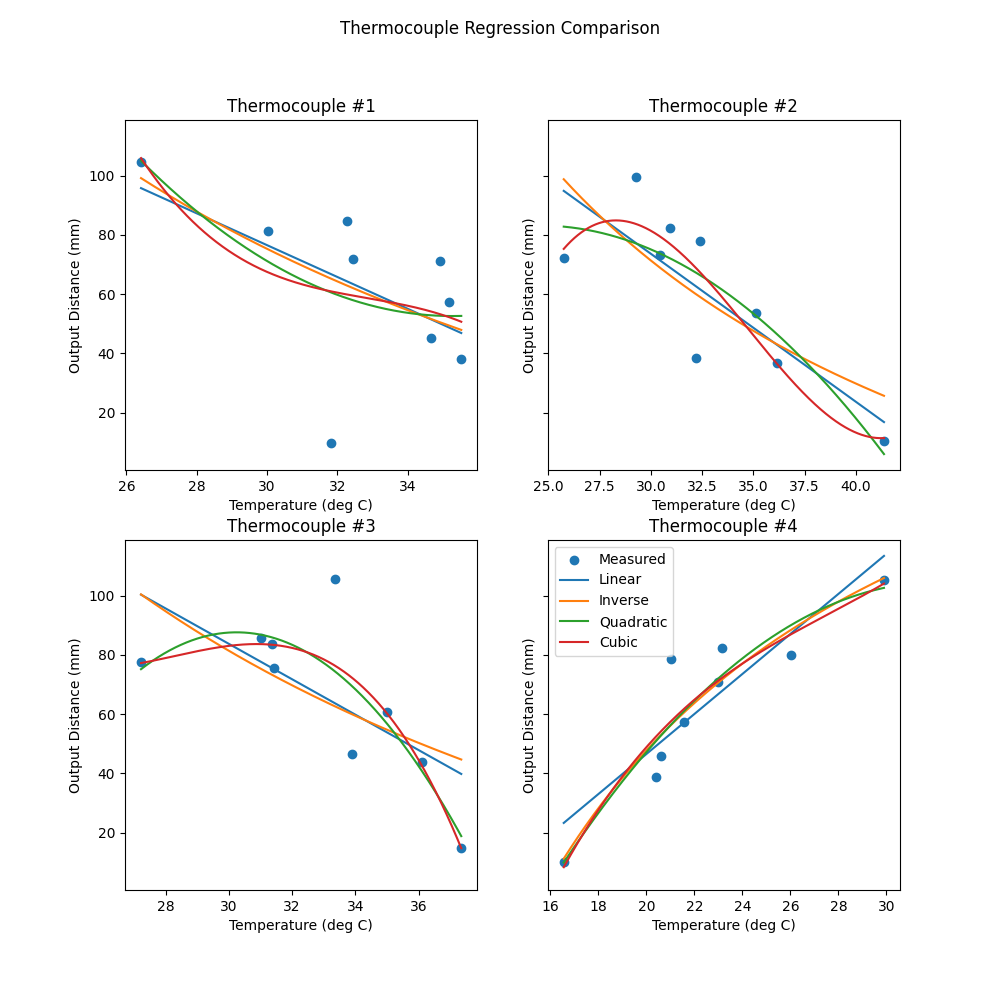
\includegraphics[width=\linewidth]{images/Thermocouple Regressions.png}
    \caption{Thermocouple Regression Comparison}
    \label{fig:compare-tc} % Label is defined below the content, to place it below the image.
\end{figure}

The cubic model had the highest coefficient of determination of the functions tested across all 4 thermocouples. By inspecting the plots however, it is clear that the relationship between temperature and distance has a large amount of variance and given the low number of sample points used to fit these models, the higher order functions are likely over-fit to the training data and would not generalize well to the test data. It was therefore decided that a linear model would be used for the thermocouples, as it is the simplest model and provides a reasonable approximation of the other models in the range of the training set data. Figure \ref{fig:fit-tc} shows the linear regression and resultant parameters.

\begin{figure}[H]
    \centering
    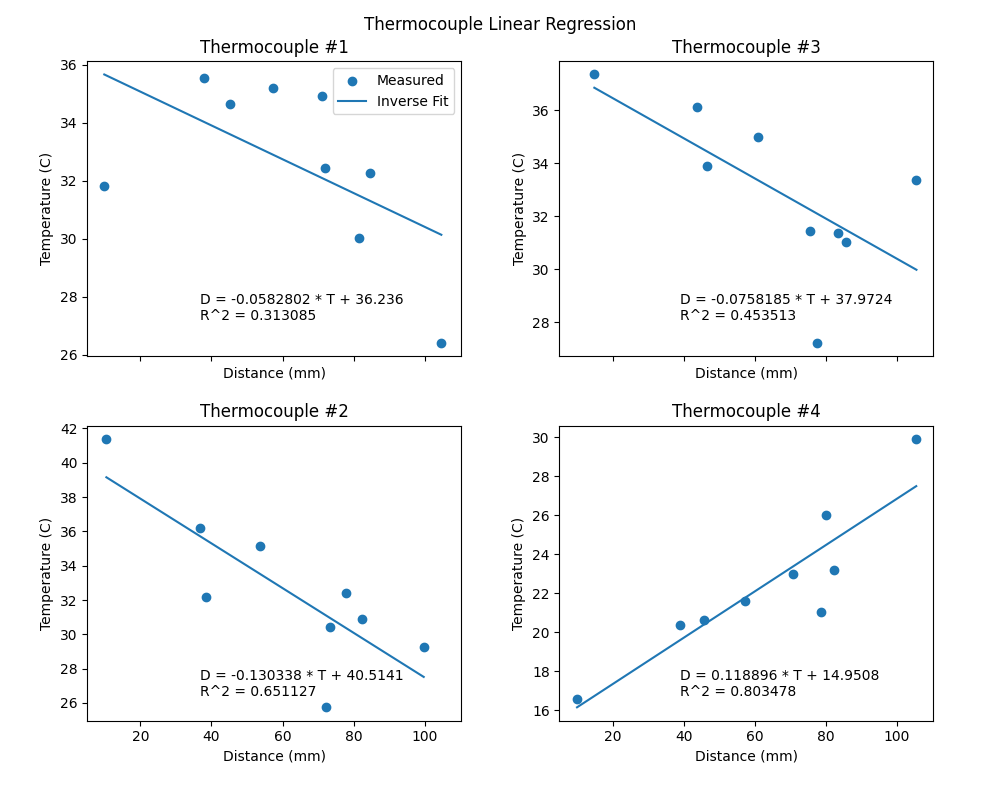
\includegraphics[width=\linewidth]{images/Thermocouple Sensor Fits.png}
    \caption{Thermocouple Regression to Linear Relationship}
    \label{fig:fit-tc} % Label is defined below the content, to place it below the image.
\end{figure}

% Model Calibration ──────────────────────────────────────────────────────────────── %

\section{Model Calibration}

Figure \ref{fig:P1} below shows the distributions of the estimated distance to the heat source for training position 1 at coordinates $[7.4, 0.6]$. The IR x-axis measurements were inaccurate registering a mean distance of 1.62cm compared to the actual 7.4cm. The IR y-axis measurements were far better at 0.46cm compared to the actual 0.6cm. Thermocouple 1 registered a much larger distance considering the Peltier module was placed directly on top of it. Thermocouples 2 and 4 had acceptable distributions whereas Thermocouple 3 measured long.

Figure \ref{fig:P3} shows the distributions of the estimated distance to the heat source for training position 3 at coordinates $[0.012, 0.05]$. At this position both IR axis measured incorrect values with an x-axis mean of -0.84cm and a y-axis mean of 11.1cm. Similar to the first case where the thermocouple closest to the heat source registered a distance much further than the actual value, thermocouple 2 detected the heat source at a distance of 3.0cm in contrast to the actual 0cm distance. Once again, thermocouple 3 measures inaccurately this time falling short by 1.3cm. Thermocouple 1 was very accurate with an error of 0.1cm and Thermocouple 4 was similarly accurate with an average distance of 6.2cm for an actual distance of 6.0cm.

Figure \ref{fig:P7} shows the distributions of the estimated distance to the heat source for training position 7 at coordinates $[7.2, 7.3]$. Once again, neither x-axis IR sensor determined accurate results leading to an off plot distribution. The y-axis IR sensors recorded a mean distance of 5.63cm, error of 1.57cm. This is the lowest error for the IR sensors among the samples shown. In this position thermocouple 3 had an actual distance of 0cm but recorded a mean distance of 3.59cm continuing the trend from the previous two positions. Thermocouple 1 possessed an error of 0.98cm, thermocouple 2 possessed an error of 2.16cm, and thermocouple 3 possessed an error of 1.21cm.

Figure Figure \ref{fig:P9} shows the distributions of the estimated distance to the heat source for training position 7 at coordinates $[0.8, 7.5]$. Neither axis IR sensors determined an accurate reading for this position. Thermocouple 4 which should have determined a position of 0cm, instead returned a distance of 5.03cm. This trend implies that the linear model implemented to convert temperature measured by the thermocouples to distance from the heat source breaks down at higher temperatures. Thermocouple 1 had an error of 0.47cm, thermocouple 2 had an error of 0.37cm, and thermocouple 3 had an error of 2.33cm.

% POSITION 1 FIGURES
\begin{figure}[H]
    \centering
    \begin{subfigure}[h]{0.8\textwidth}
        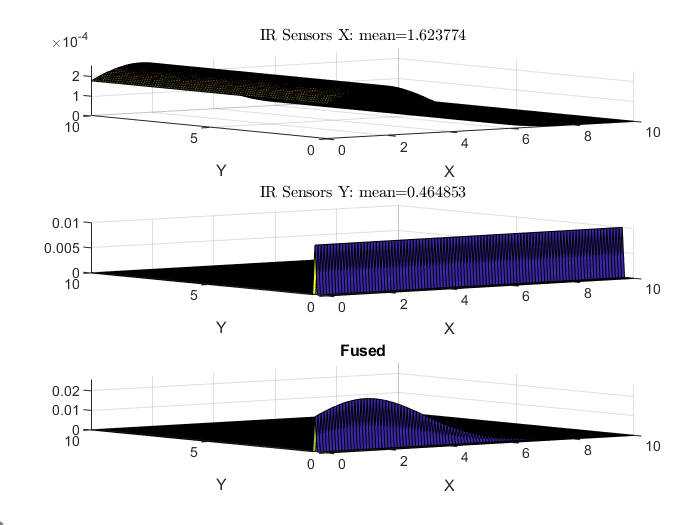
\includegraphics[width=\textwidth]{images/P1.png}
        \caption{IR Sensors at Position 1}
        \label{fig:P1IR}
    \end{subfigure}
    \vskip0.5\baselineskip
    \begin{subfigure}[h]{0.4\textwidth}
        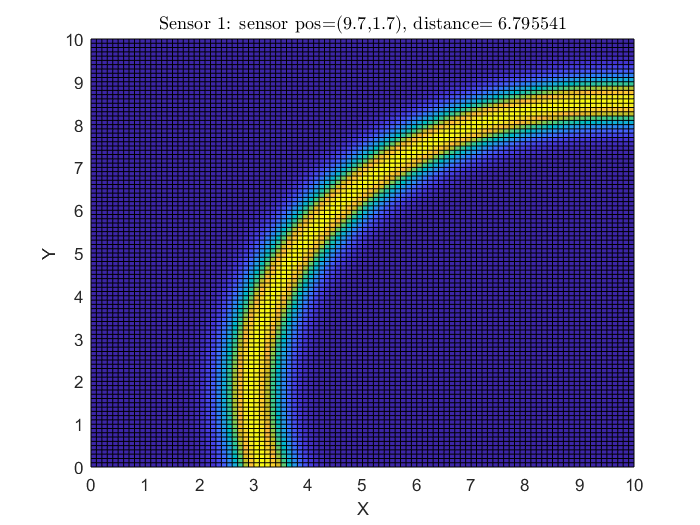
\includegraphics[width=\textwidth]{images/P1S1.png}
        \caption{Thermocouple 1 at Position 1}
        \label{fig:P1S1}
    \end{subfigure}
    \begin{subfigure}[h]{0.4\textwidth}
        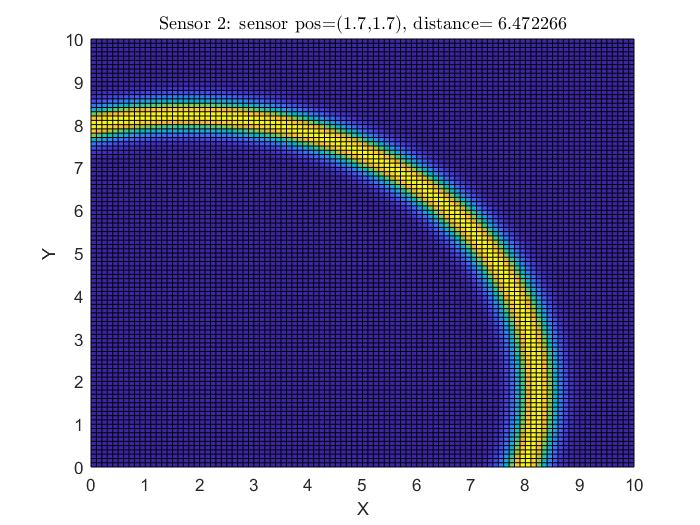
\includegraphics[width=\textwidth]{images/P1S2.png}
        \caption{Thermocouple 2 at Position 1}
        \label{fig:P1S2}
    \end{subfigure}
    \vskip0.5\baselineskip
    \begin{subfigure}[h]{0.4\textwidth}
        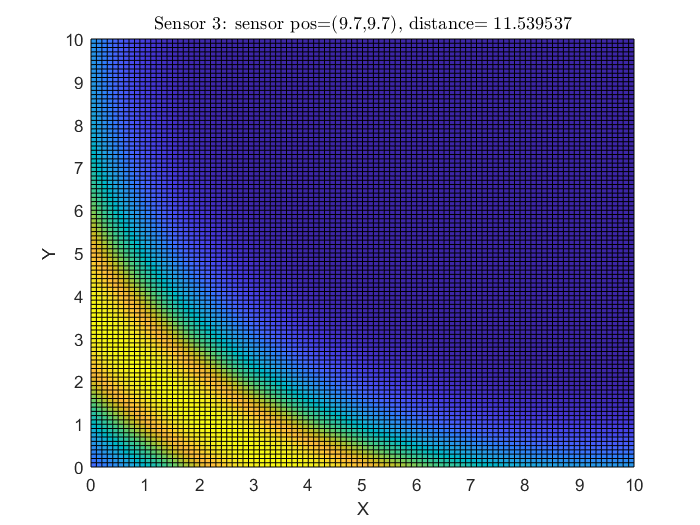
\includegraphics[width=\textwidth]{images/P1S3.png}
        \caption{Thermocouple 3 at Position 1}
        \label{fig:P1S3}
    \end{subfigure}
    \begin{subfigure}[h]{0.4\textwidth}
        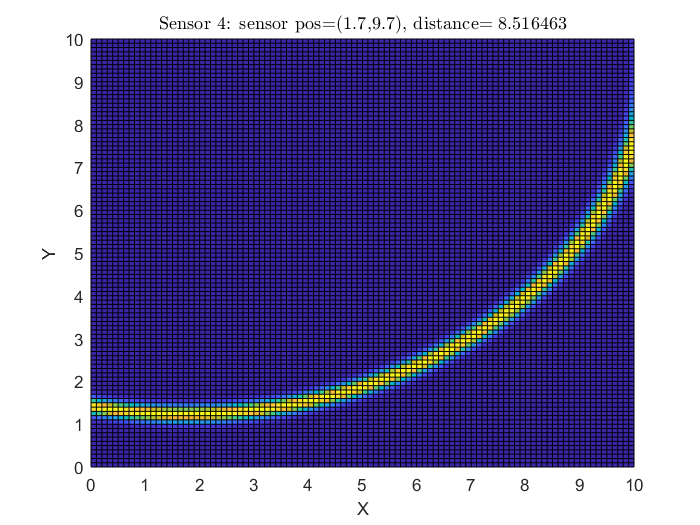
\includegraphics[width=\textwidth]{images/P1S4.png}
        \caption{Thermocouple 4 at Position 1}
        \label{fig:P1S4}
    \end{subfigure}
\caption{Position 1 Thermocouple Readings}
\label{fig:P1}
\end{figure}

% POSITION 3 FIGURES
\begin{figure}[H]
    \centering
    \begin{subfigure}[h]{0.8\textwidth}
        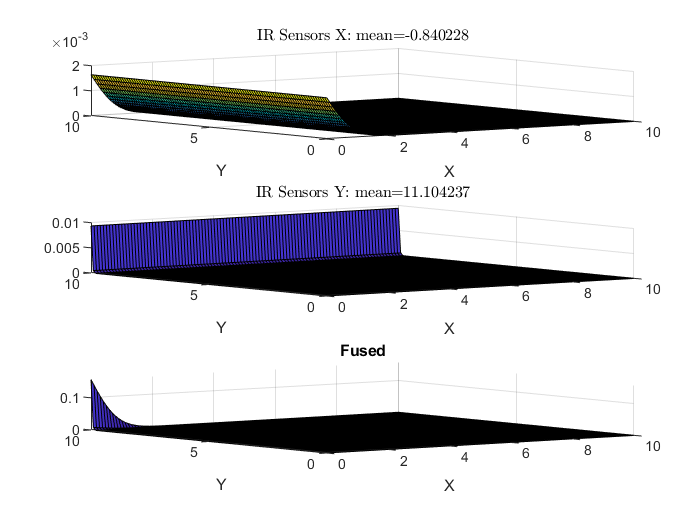
\includegraphics[width=\textwidth]{images/P3.png}
        \caption{IR Sensors at Position 3}
        \label{fig:P3IR}
    \end{subfigure}
    \vskip0.5\baselineskip
    \begin{subfigure}[h]{0.4\textwidth}
        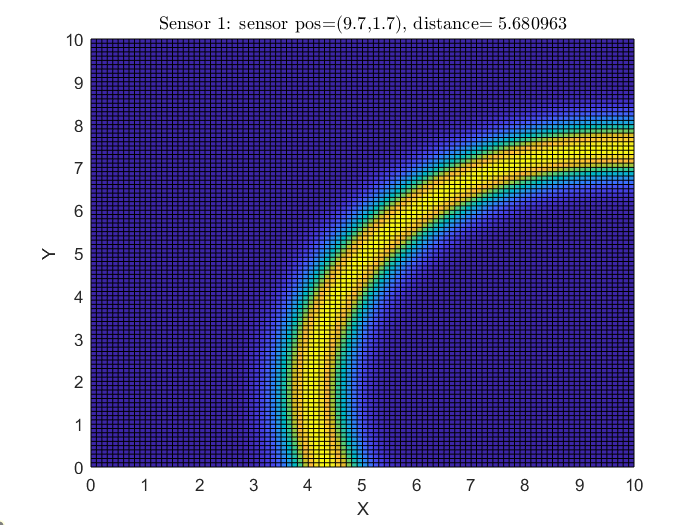
\includegraphics[width=\textwidth]{images/P3S1.png}
        \caption{Thermocouple 1 at Position 3}
        \label{fig:P3S1}
    \end{subfigure}
    \begin{subfigure}[h]{0.4\textwidth}
        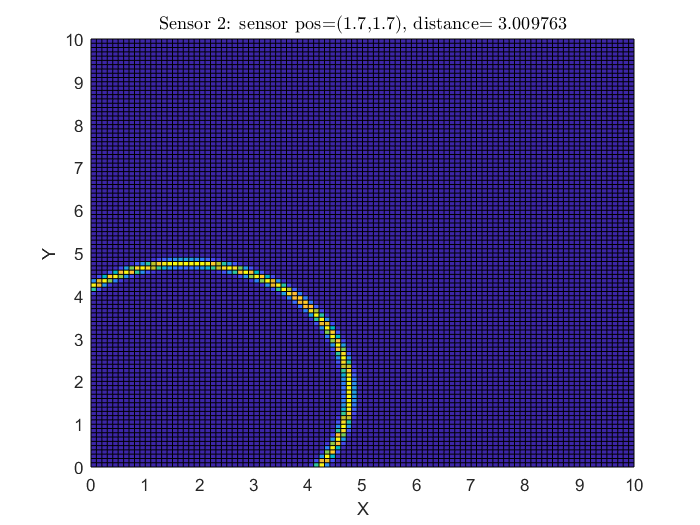
\includegraphics[width=\textwidth]{images/P3S2.png}
        \caption{Thermocouple 2 at Position 3}
        \label{fig:P3S2}
    \end{subfigure}
    \vskip0.5\baselineskip
    \begin{subfigure}[h]{0.4\textwidth}
        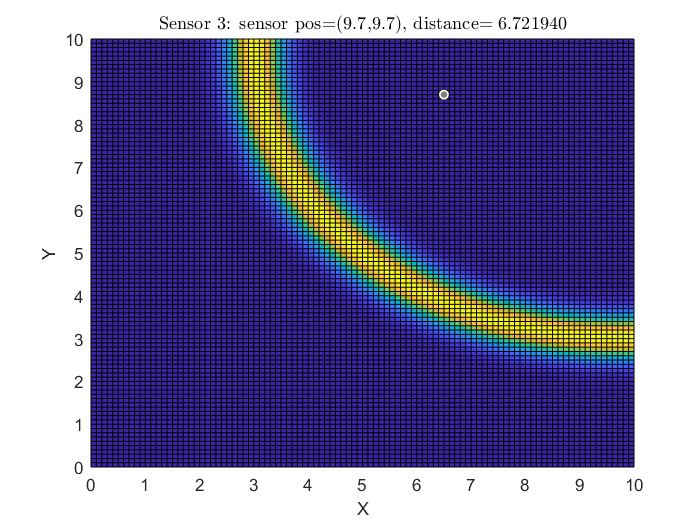
\includegraphics[width=\textwidth]{images/P3S3.png}
        \caption{Thermocouple 3 at Position 3}
        \label{fig:P3S3}
    \end{subfigure}
    \begin{subfigure}[h]{0.4\textwidth}
        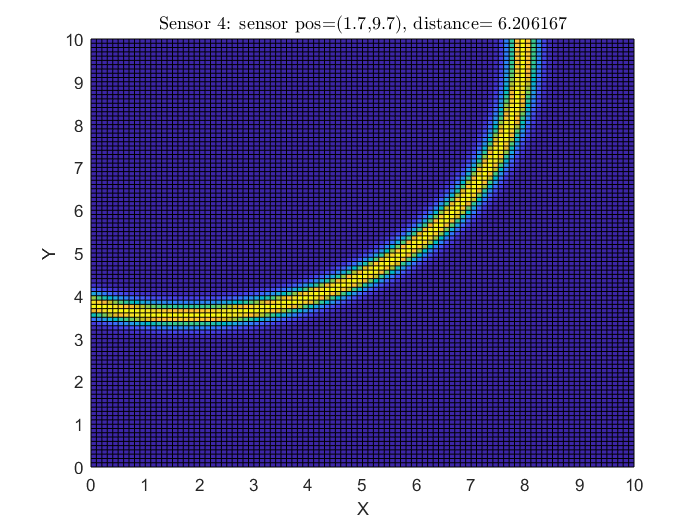
\includegraphics[width=\textwidth]{images/P3S4.png}
        \caption{Thermocouple 4 at Position 3}
        \label{fig:P3S4}
    \end{subfigure}
\caption{Position 3 Thermocouple Readings}
\label{fig:P3}
\end{figure}

% POSITION 7 FIGURES
\begin{figure}[H]
    \centering
    \begin{subfigure}[h]{0.8\textwidth}
        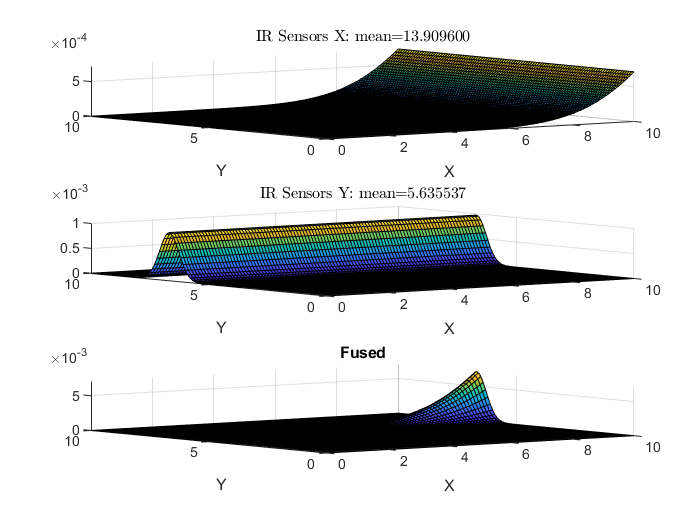
\includegraphics[width=\textwidth]{images/P7.png}
        \caption{IR Sensors at Position 7}
        \label{fig:P7IR}
    \end{subfigure}
    \vskip0.5\baselineskip
    \begin{subfigure}[h]{0.4\textwidth}
        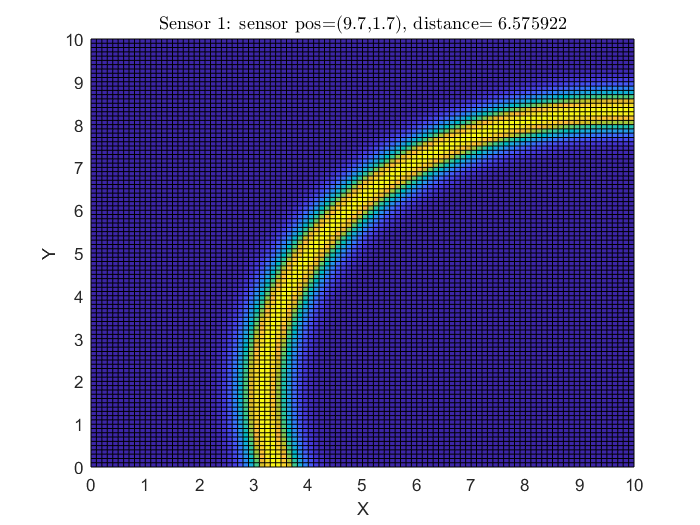
\includegraphics[width=\textwidth]{images/P7S1.png}
        \caption{Thermocouple 1 at Position 7}
        \label{fig:P7S1}
    \end{subfigure}
    \begin{subfigure}[h]{0.4\textwidth}
        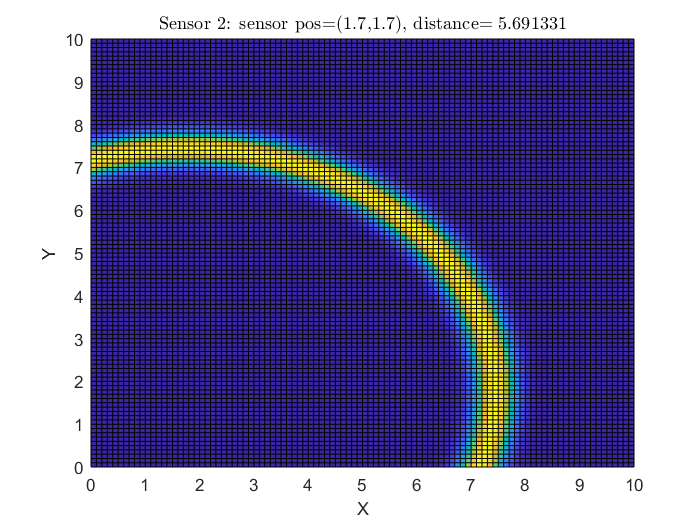
\includegraphics[width=\textwidth]{images/P7S2.png}
        \caption{Thermocouple 2 at Position 7}
        \label{fig:P7S2}
    \end{subfigure}
    \vskip0.5\baselineskip
    \begin{subfigure}[h]{0.4\textwidth}
        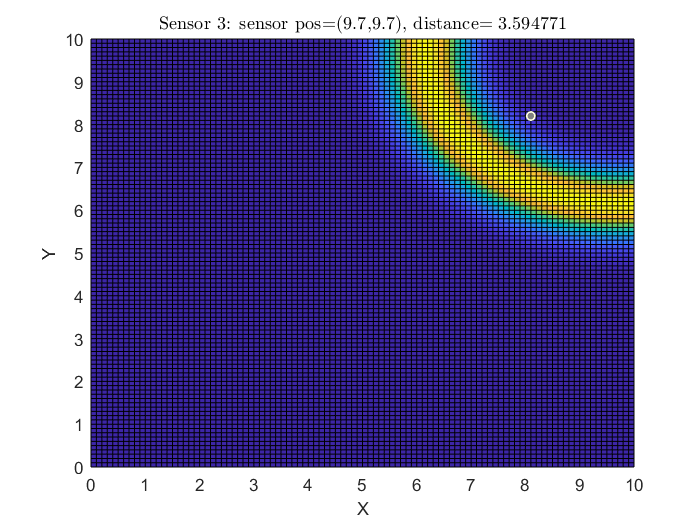
\includegraphics[width=\textwidth]{images/P7S3.png}
        \caption{Thermocouple 3 at Position 7}
        \label{fig:P7S3}
    \end{subfigure}
    \begin{subfigure}[h]{0.4\textwidth}
        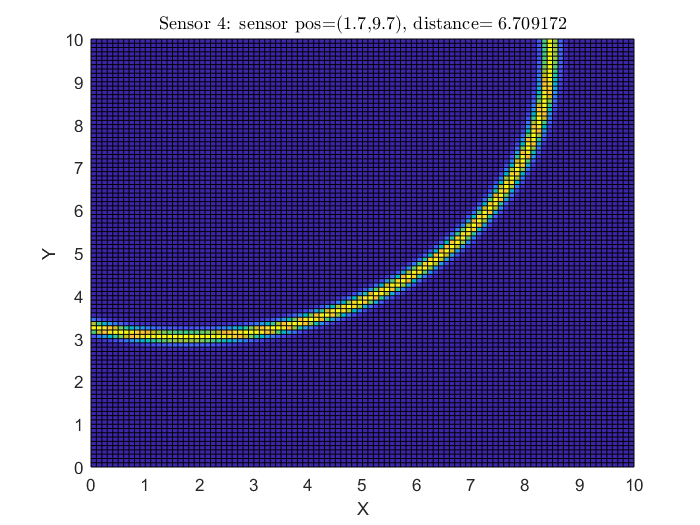
\includegraphics[width=\textwidth]{images/P7S4.png}
        \caption{Thermocouple 4 at Position 7}
        \label{fig:P7S4}
    \end{subfigure}
\caption{Position 7 Thermocouple Readings}
\label{fig:P7}
\end{figure}

% POSITION 9 FIGURES
\begin{figure}[H]
    \centering
    \begin{subfigure}[h]{0.8\textwidth}
        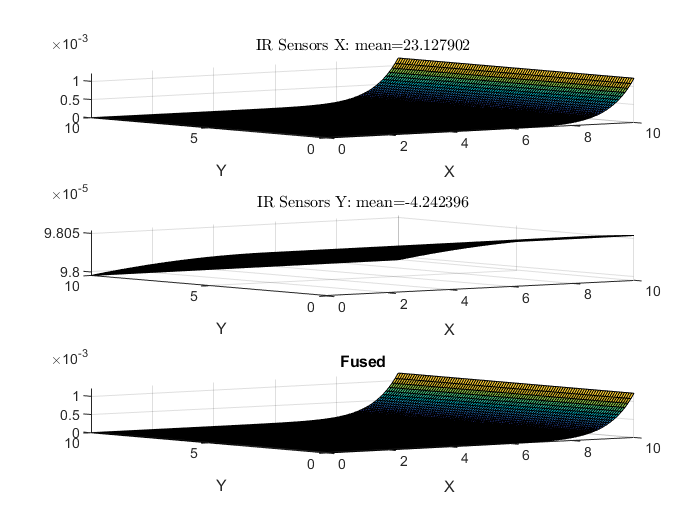
\includegraphics[width=\textwidth]{images/P9.png}
        \caption{IR Sensors at Position 9}
        \label{fig:P9IR}
    \end{subfigure}
    \vskip0.5\baselineskip
    \begin{subfigure}[h]{0.4\textwidth}
        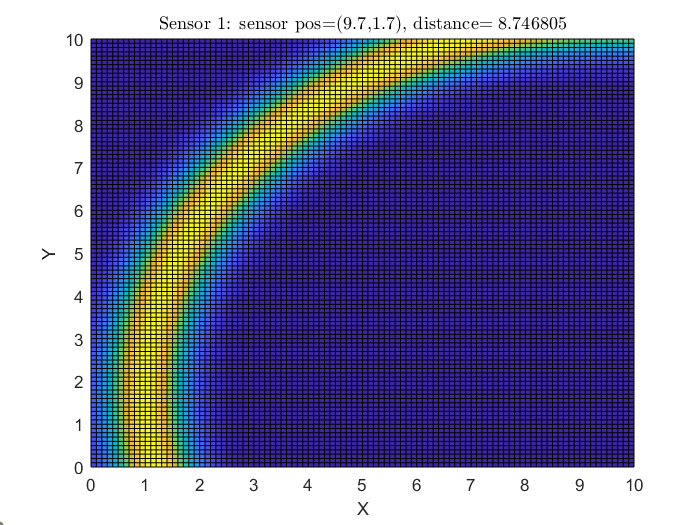
\includegraphics[width=\textwidth]{images/P9S1.png}
        \caption{Thermocouple 1 at Position 9}
        \label{fig:P9S1}
    \end{subfigure}
    \begin{subfigure}[h]{0.4\textwidth}
        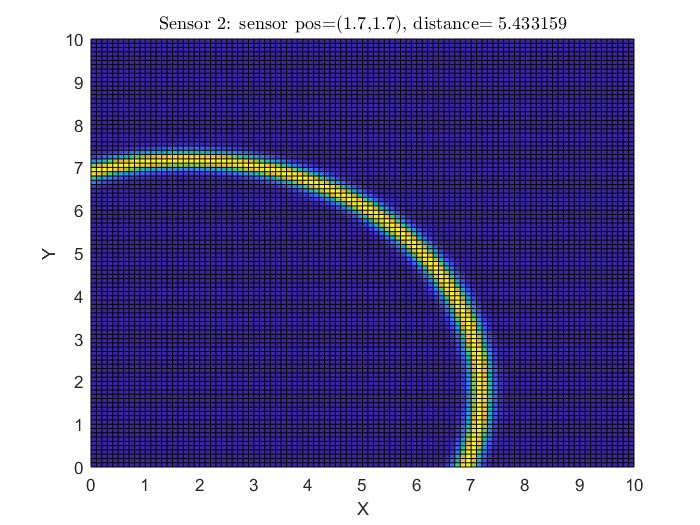
\includegraphics[width=\textwidth]{images/P9S2.png}
        \caption{Thermocouple 2 at Position 9}
        \label{fig:P9S2}
    \end{subfigure}
    \vskip0.5\baselineskip
    \begin{subfigure}[h]{0.4\textwidth}
        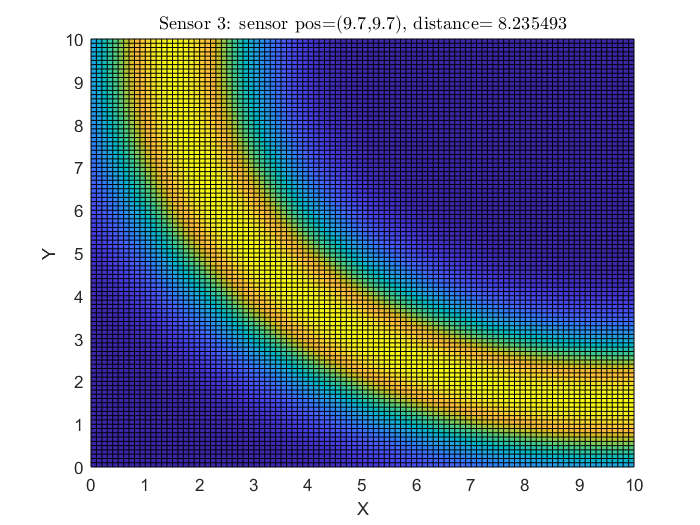
\includegraphics[width=\textwidth]{images/P9S3.png}
        \caption{Thermocouple 3 at Position 9}
        \label{fig:P9S3}
    \end{subfigure}
    \begin{subfigure}[h]{0.4\textwidth}
        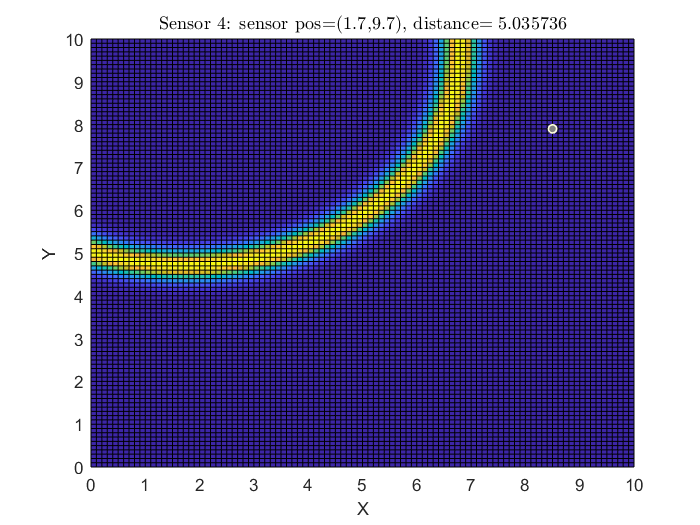
\includegraphics[width=\textwidth]{images/P9S4.png}
        \caption{Thermocouple 4 at Position 9}
        \label{fig:P9S4}
    \end{subfigure}
\caption{Position 9 Thermocouple Readings}
\label{fig:P9}
\end{figure}

% Sensor Evalutation ──────────────────────────────────────────────────────────────── %

\section{Model Evaluation}

\subsection{IR Sensor Fusion}
Using only the IR sensors, the positions of each of the test points was estimated. The probability distributions are shown in figure \ref{fig:IR-Fus}. In an attempt to improve the results, the IR sensor data was tested before being utilized in the model. Due to the positioning of the block in certain positions, it may not have been visible to one of the IR sensors. To account for this, the mean distance values were analyzed. In the case where both sensors  registered the block at a distance within the range of the test area, Bayesian fusion was performed to fuse the data from both sensors. In a case where one sensor did not detect the block within the test area, the distribution of the other sensor was used. In the case where neither sensor detected the block within the test area, the sensor with the better reading was used. Despite this effort, the model still appears to perform rather poorly. Test point 1 in figure \ref{fig:IR-Fus-1} is predicted to be in the corner of the plate at $[10, 0]$, near training point 1 (refer to table \ref{tab:layout}). The actual location of test point 1 was $[5.5, 2.4]$. The predicted position of point 2 shows to be roughly $[0, 5]$, far from the measured $[1.9, 4.0]$, but relatively close in the Y direction. This is likely due to the long range IR sensors measuring in the X direction not seeing the block, therefore registering an invalid distance that is corrected by the filtering to be 0. The short range sensors are able to pick up the block and do a decent job of providing an accurate measurement. Test point 3 is also predicted to be in the $[10, 0]$ corner. With a measured position of $[5.5, 7.0]$, the IR sensors again fail to correctly place the block on the plate. Overall, the performance of the IR model alone is very poor, failing to accurately measure the blocks position in 7 of 8 cases.

% IR Sensor Fusion
\begin{figure}[H]
    \centering
    \begin{subfigure}[h]{0.45\textwidth}
        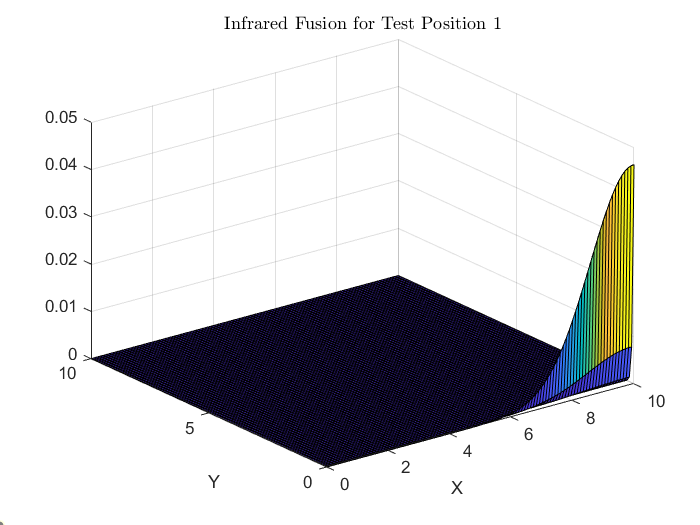
\includegraphics[width=\textwidth]{images/IR_FusionA1.png}
        \caption{Test Point 1}
        \label{fig:IR-Fus-1}
    \end{subfigure}
    \begin{subfigure}[h]{0.45\textwidth}
        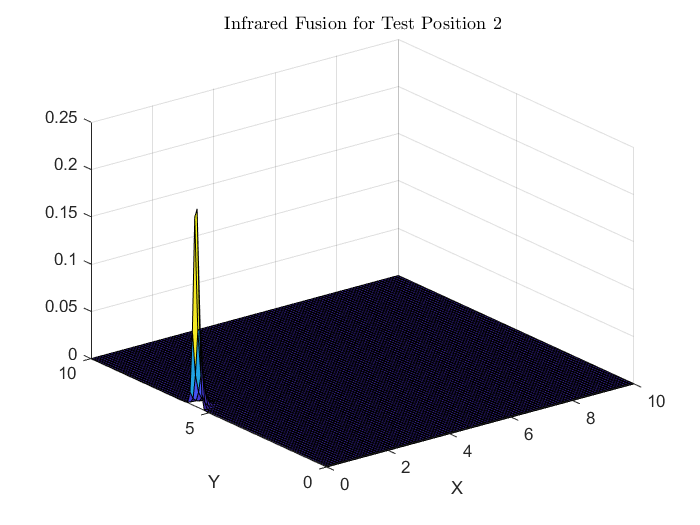
\includegraphics[width=\textwidth]{images/IR_FusionA2.png}
        \caption{Test Point 2}
        \label{fig:IR-Fus-2}
    \end{subfigure}
    \begin{subfigure}[h]{0.45\textwidth}
        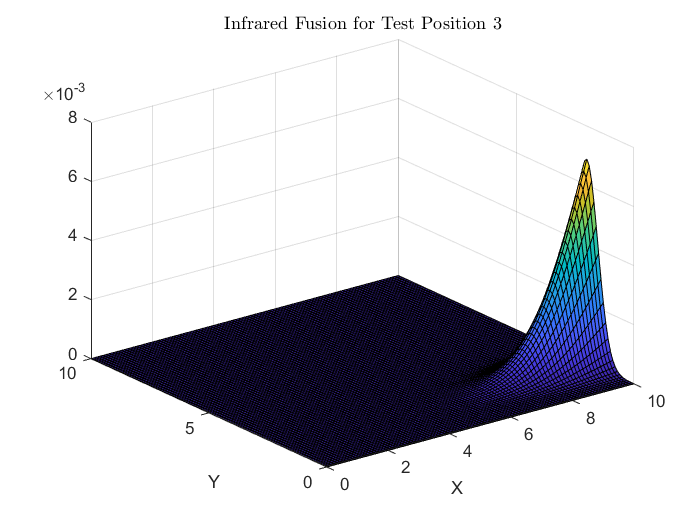
\includegraphics[width=\textwidth]{images/IR_FusionA3.png}
        \caption{Test Point 3}
        \label{fig:IR-Fus-3}
    \end{subfigure}
    \caption{IR Fusion Readings}
    \label{fig:IR-Fus}
\end{figure}

\subsection{Thermocouple Sensor Fusion}

Using only the thermocouple sensors, the positions of each of the test points was estimated. The probability distributions are shown in figure \ref{fig:TC-Fus}. The distributions show promising results, producing 3 specific points of likelihood for the measured test points. Test point 1, measured at $[5.5, 2.4]$ is predicted to be at roughly $[7.9, 4.1]$. This measurement is within the margin of error of the blocks width. Accounting for the blocks dimensions of 3cmx3cm, the measured position is within 1cm of the blocks center in both the X and Y directions. Test point 2 measured at $[1.9, 4.0]$ is predicted to be at $[6.5, 4.5]$. The X measurement is wildly incorrect, predicting the wrong side of the plate, while the Y measurement is accurate to within 0.5cm. Test point 3 measured at $[5.5, 7.0]$ is predicted to be at $[7.0, 6.4]$. In this case, accounting for the blocks dimensions, puts the X prediction perfectly in line but the Y prediction 3cm off. Overall, sensor fusion from the thermocouples alone is not a reliable method of location the block and Peltier cell on the plate.

% Thermocouple Sensor Fusion
\begin{figure}[H]
    \centering
    \begin{subfigure}[h]{0.45\textwidth}
        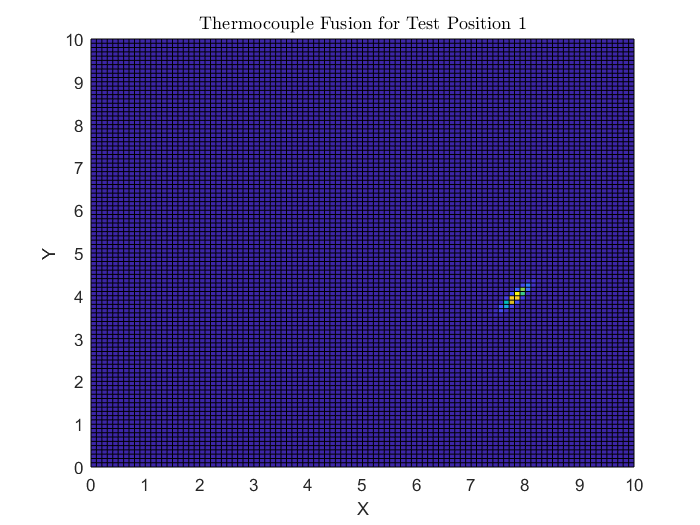
\includegraphics[width=\textwidth]{images/ThermocoupleFusionA1.png}
        \caption{Test Point 1}
        \label{fig:TC-Fus-1}
    \end{subfigure}
    \begin{subfigure}[h]{0.45\textwidth}
        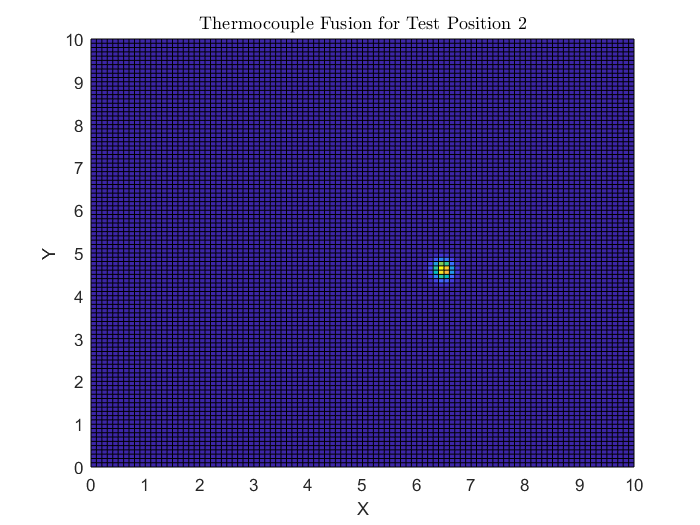
\includegraphics[width=\textwidth]{images/ThermocoupleFusionA2.png}
        \caption{Test Point 2}
        \label{fig:TC-Fus-2}
    \end{subfigure}
    \begin{subfigure}[h]{0.45\textwidth}
        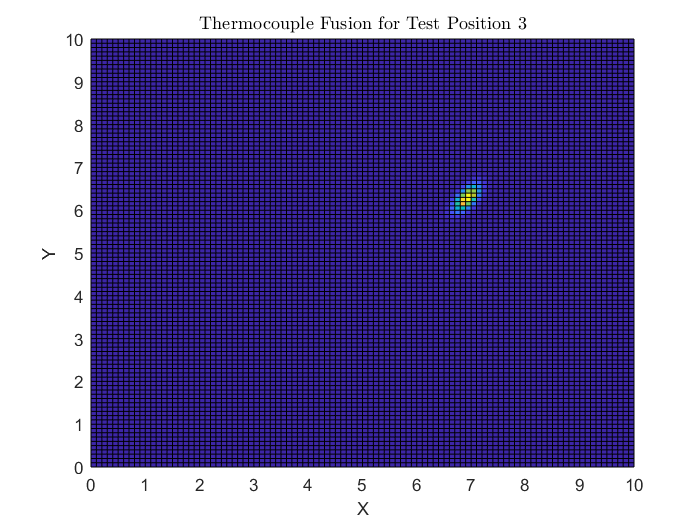
\includegraphics[width=\textwidth]{images/ThermocoupleFusionA3.png}
        \caption{Test Point 3}
        \label{fig:TC-Fus-3}
    \end{subfigure}
    \caption{Thermocouple Fusion Readings}
    \label{fig:TC-Fus}
\end{figure}

\subsection{Infrared and Thermocouple Sensor Fusion}

% IR + Thermocouple Sensor Fusion
\begin{figure}[H]
    \centering
    \begin{subfigure}[h]{0.45\textwidth}
        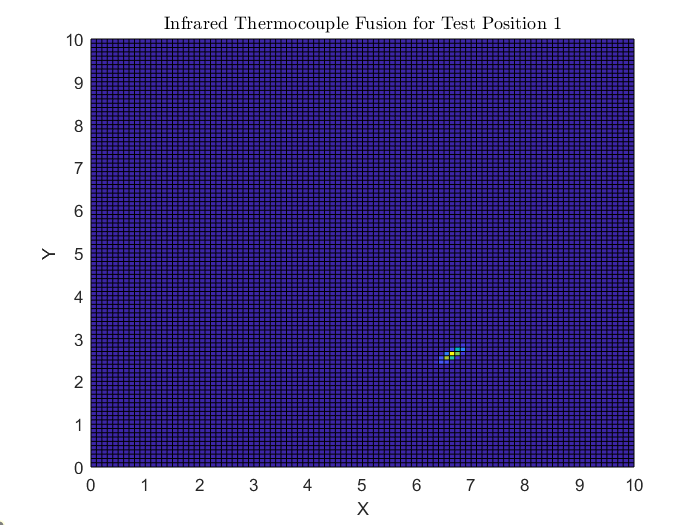
\includegraphics[width=\textwidth]{images/IR_TempFusionA1.png}
        \caption{Test Point 1}
        \label{fig:Fus-1}
    \end{subfigure}
    \begin{subfigure}[h]{0.45\textwidth}
        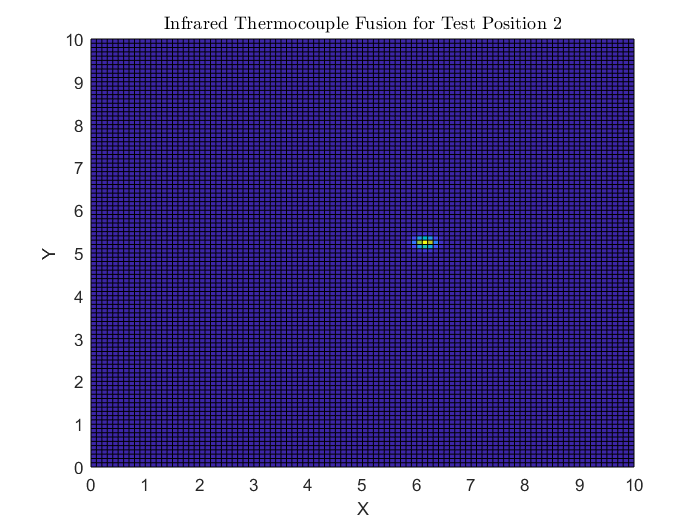
\includegraphics[width=\textwidth]{images/IR_TempFusionA2.png}
        \caption{Test Point 2}
        \label{fig:Fus-2}
    \end{subfigure}
    \begin{subfigure}[h]{0.45\textwidth}
        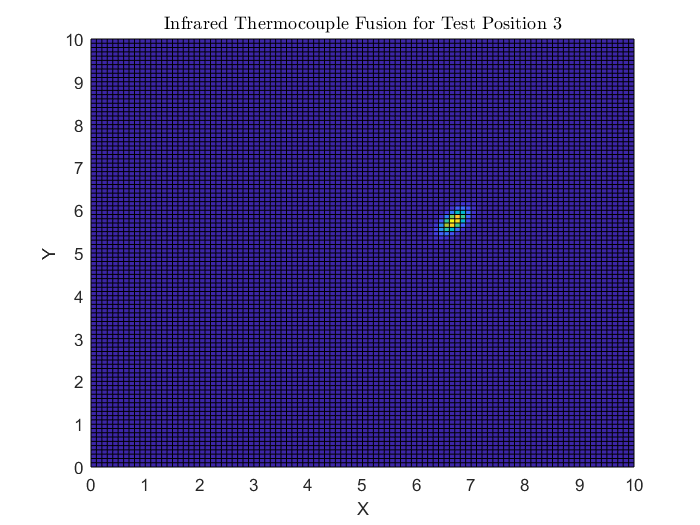
\includegraphics[width=\textwidth]{images/IR_TempFusionA3.png}
        \caption{Test Point 3}
        \label{fig:Fus-3}
    \end{subfigure}
    \caption{IR and Thermocouple Fusion Readings}
    \label{fig:Fus}
\end{figure}
Figure \ref{fig:Fus} above shows the combined fusion between the IR sensors and the thermocouples for the three test points. The fusion of the sensors provided a very small distribution for each of these points indicating that there was very little overlap between each of the distributions involved. Test position 1 was estimated to be at coordinates $[6.7, 2.7]$. The measured position was $[5.5, 2.4]$. This equates to an error of 1.29cm. Test position 2 was estimated to be at coordinates $[6.1, 5.4]$. Comparing this to the measured coordinates of $[1.9, 4.0]$ results in an error of 4.43cm, significantly larger. Test position 3 was estimated to be at coordinates $[6.7, 5.7]$. It was measured at a position of $[5.5, 7.0]$ resulting in an error of 1.77cm. While the fusion of these sensors provided a highly consistent result, it was an inaccurate one. Likely with superior IR data the result could have been greatly improved. 
The advantage of performing this type of sensor fusion is a more reliable result is achieved through the consideration of multiple sensors recording different types of data. The multiplication of valid gaussian probability distributions results in a higher certainty of measurements, as was seen with the thermocouples. The disadvantage is that there is no benefit when the measurements of the sensors are inconsistent with one another as seen with the IR sensors. Since both sensors in the same axis often differed significantly in their measurements, the only thing that could be done was to take the better of the two sets which resulted in highly unreliable results. 

% REFERENCES ──────────────────────────────────────────────────────────────── %
\clearpage
\bibliographystyle{plain} % We choose the "plain" reference style
\bibliography{references} % Entries are in the references.bib file

% APPENDIX ──────────────────────────────────────────────────────────────── %
\clearpage
\section{Appendix} \label{appendix}

\subsection{Full Code Listings}
% Solvy_boi.py
\lstinputlisting[title=\texttt{\scriptsize Sensor-Calibration.py},
                 caption=Sensor Calibration Script | Sensor-Calibration.py,
                 label=lst:sensor-calibration-source]{./Sensor-Calibration.py}
\clearpage

\end{document}
